\input templates/header

\usepackage{epigraph}
\usepackage{listings}
\usepackage{colortbl}

\lstset{
  basicstyle=\ttfamily,
  columns=fullflexible,
		keepspaces=true,
  keywordstyle=\color{red}\bfseries,
  commentstyle=\color{blue},
  showstringspaces=false,
  language=c++,
  tabsize=4,
}

\newcommand{\Sum}{\mathit{sum}}
\newcommand{\MaxSoFar}{\mathit{maxSoFar}}
\newcommand{\MaxEndingHere}{\mathit{maxEndingHere}}

\newcommand*{\RC}[1]{\hfill\makebox[3.0cm][l]{#1}}%


\title[ASD - Introduzione]{\textbf{Algoritmi e Strutture Dati}\\[24pt]Introduzione al corso}

\graphicspath{{figs/00/}}

\begin{document}

%-------------------------------------------------------------------------
\FrameTitle{}

%-------------------------------------------------------------------------
\begin{frame}{Cos'è un informatico?}
\IG{0.5}{geek.jpg}
\end{frame}

%-------------------------------------------------------------------------
\begin{frame}{Colloquio di lavoro}
	
\vspace{-9pt}
\begin{myboxtitle}[Problema: Sottovettore di somma massimale]
\BI
\item \textbf{Input}: un vettore di interi $A[1 \ldots n]$
\item \textbf{Output}: il sottovettore $A[i \ldots j]$ di somma massimale,
ovvero il sottovettore la cui somma degli elementi $\sum_{k=i}^j A[k]$ è
più grande o uguale alla somma degli elementi di qualunque altro sottovettore.
\EI
\end{myboxtitle}
\end{frame}

%-------------------------------------------------------------------------
\begin{frame}{La vostra risposta}

\TwoColsCustom{0.60}{0.35}{

\includegraphics[width=\textwidth]{fig0.png}
}{
Eh?  \\(NOOB)
}	

\end{frame}

%-------------------------------------------------------------------------
\begin{frame}{La vostra risposta}
\TwoColsCustom{0.5}{0.45}{
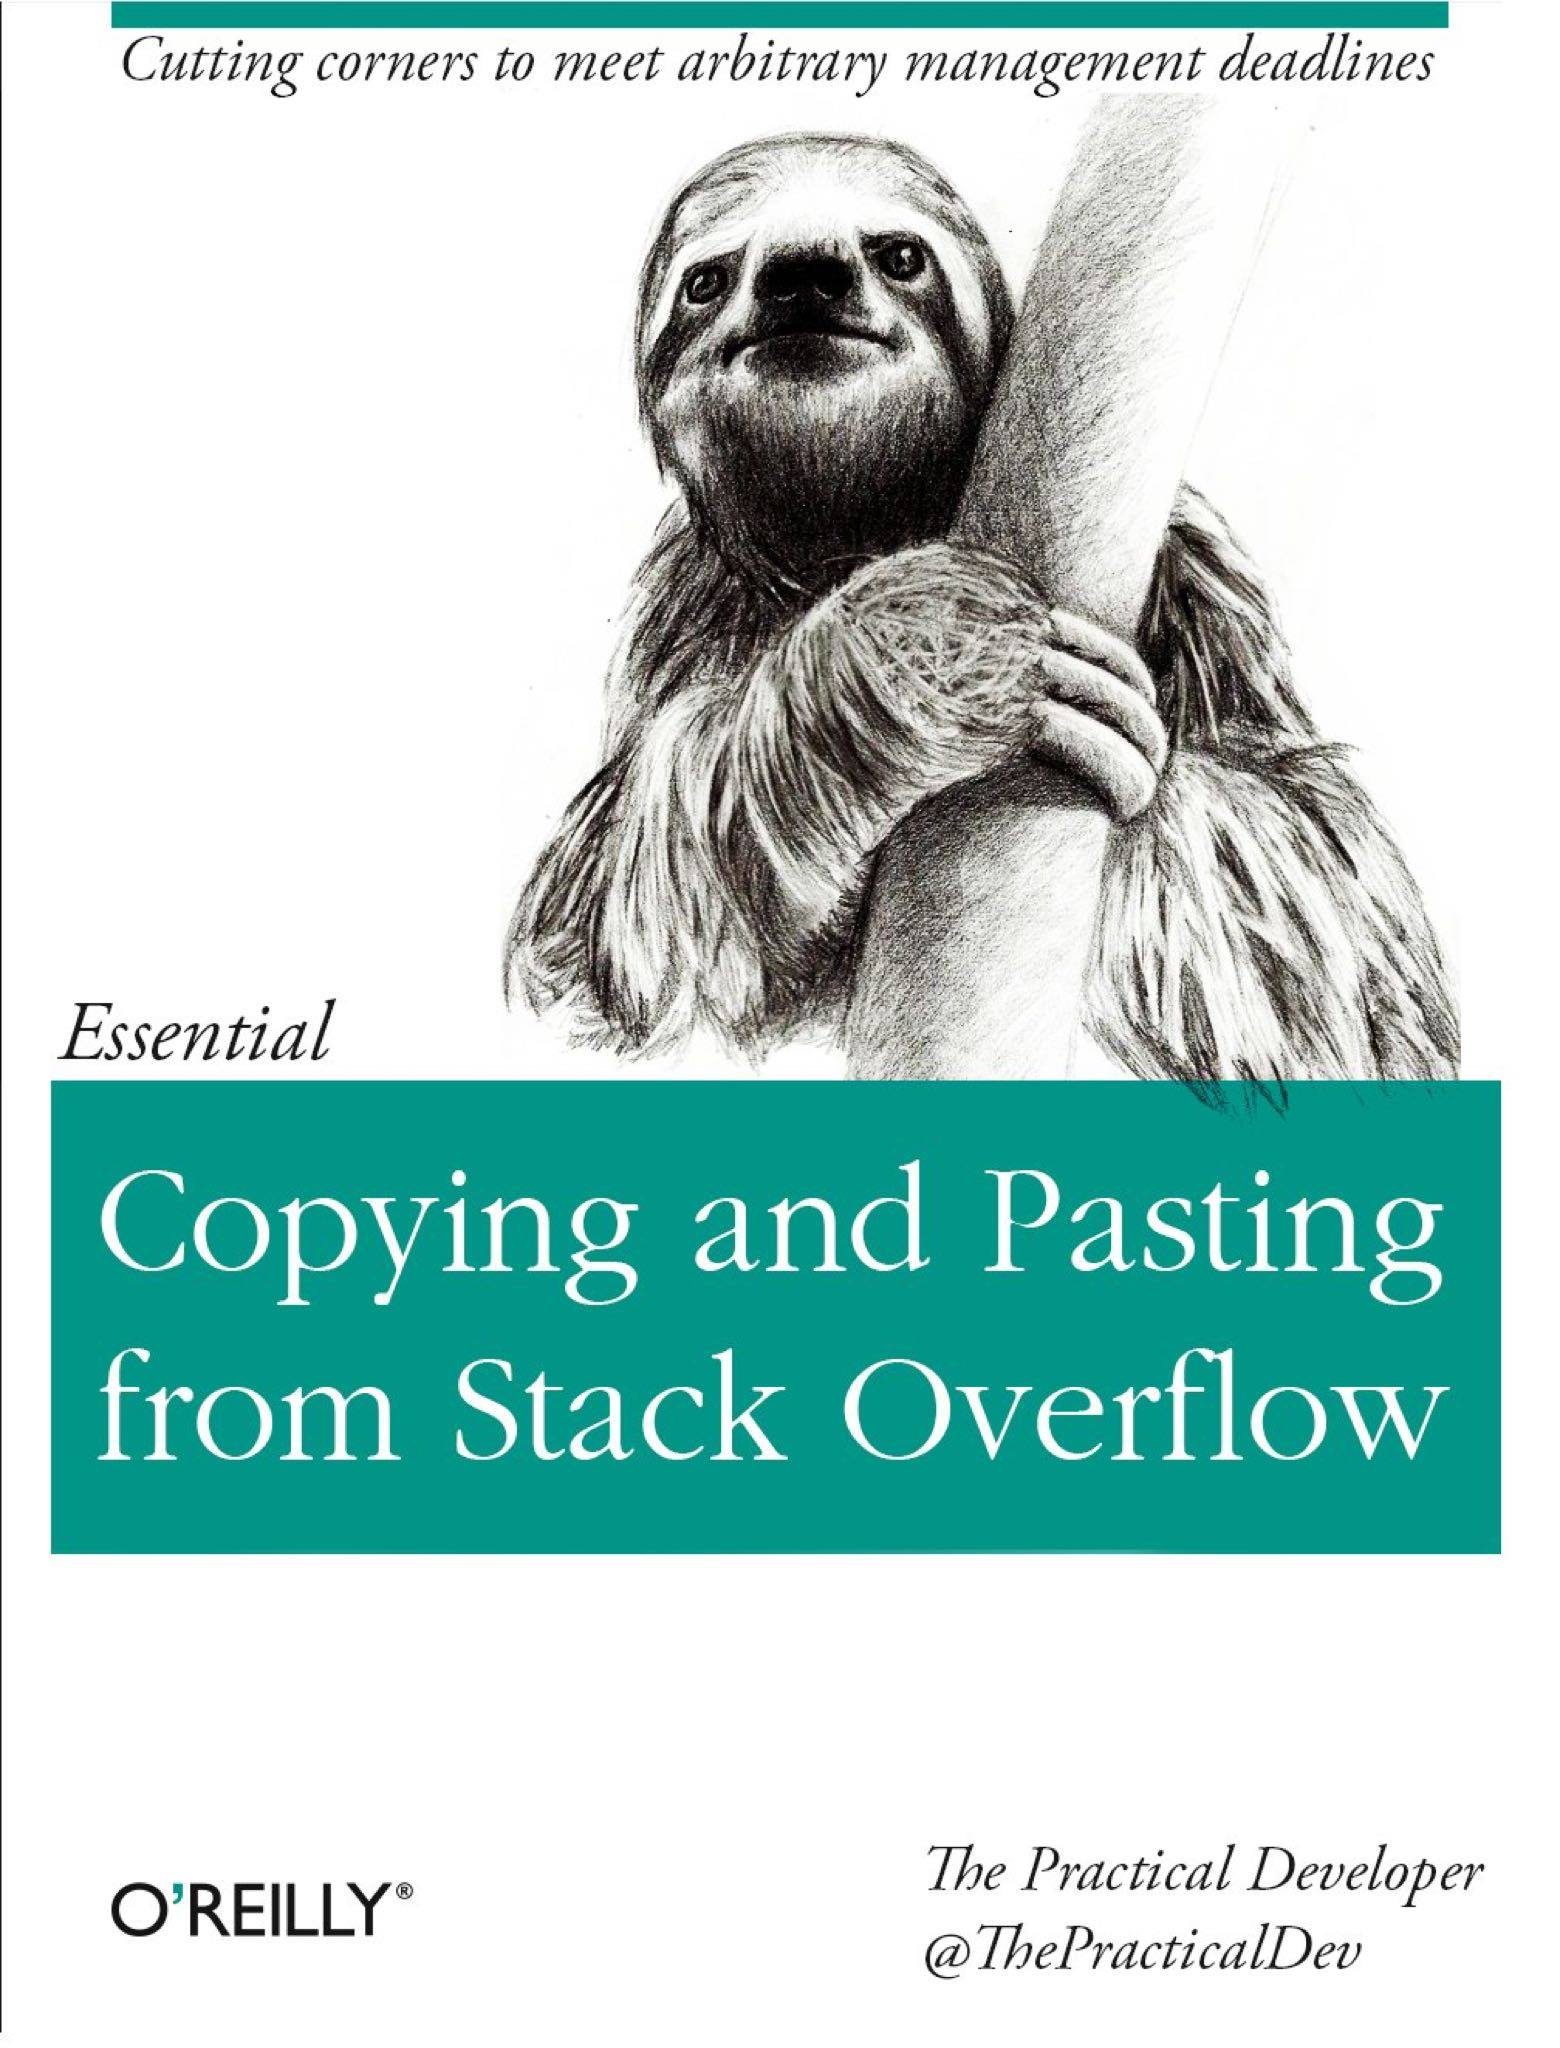
\includegraphics[width=0.8\textwidth]{stackoverflow.jpg}
}{
Posso guardare su StackOverflow?\\(CODE MONKEY)
}

%-------------------------------------------------------------------------
\end{frame}

\begin{frame}{La vostra risposta}
\TwoColsCustom{0.5}{0.45}{
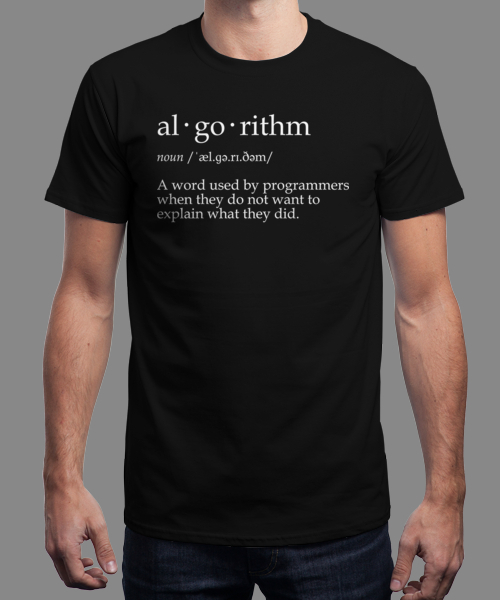
\includegraphics[width=\textwidth]{cs.jpg}
}{
Posso sviluppare un algoritmo efficiente per lei! \\(COMPUTER SCIENTIST)
}	
	
	
\end{frame}


%-------------------------------------------------------------------------
\begin{frame}[fragile]{Colloquio di lavoro}
	
\vspace{-6pt}
\begin{myboxtitle}[Problema: Sottovettore di somma massimale]
\BI
\item \textbf{Input}: un vettore di interi $A[1 \ldots n]$
\item \textbf{Output}: il sottovettore $A[i \ldots j]$ di somma massimale,
ovvero il sottovettore la cui somma degli elementi $\sum_{k=i}^j A[k]$ è
più grande o uguale alla somma degli elementi di qualunque altro sottovettore.
\EI
\end{myboxtitle}

\begin{overprint}	
\onslide<1|handout:0>
\BI
\item Il problema è descritto bene?
\EI

\onslide<2|handout:0>
\BI
\item Il problema è descritto bene?
\EI

\bigskip
\begin{center}
\begingroup
\small
\begin{tabular}{|r|r|r|r|r|r|r|r|r|r|r|r|r|r|}
\hline
      ~1 & ~3 & ~4 & -8 & ~{2} & {~3} & {-1} & {~3} & {~4} & {-3} & {10} & -3 &  2 \\\hline
\end{tabular}
\endgroup
\end{center}


\onslide<3|handout:1>
\BI
\item Il problema è descritto bene?
\EI

\bigskip
\begin{center}
\begingroup
\small
\begin{tabular}{|r|r|r|r|r|r|r|r|r|r|r|r|r|r|}
\hline
       ~1 & ~3 & ~4 & -8 & ~\cellcolor{red!30}{2} & \cellcolor{red!30}{~3} & \cellcolor{red!30}{-1} & \cellcolor{red!30}{~3} & \cellcolor{red!30}{~4} & \cellcolor{red!30}{-3} & \cellcolor{red!30}{10} & -3 &  2 \\\hline
\end{tabular}
\endgroup
\end{center}

\onslide<4|handout:2>
\BI
\item Il problema è descritto bene?
\item Riuscite a risolverlo?
\item Riuscite a risolverlo in maniera efficiente?
\EI

\end{overprint}

\end{frame}

\begin{frame}[fragile]{Utility function: Somma sottovettore}

Usiamo una funzione che dato un vettore $A$ e due indici $i$, $j$ contenuti in $A$, restituisca la somma di tutti gli elementi compresi fra $i$ e $j$ (inclusi).

\small
\begin{myboxtitle}[Java]
\vspace{-6pt}
\begin{lstlisting}{language=java}
int sum(int[] A, int i, int j) {
  int sumSoFar = 0;
  for (int k = i; k <= j; k++) {
    sumSoFar += A[k];
  }
  return sumSoFar;
}
\end{lstlisting}
\vspace{-6pt}
\end{myboxtitle}
\begin{multicols}{2}
\vspace{-6pt}
\begin{myboxtitle}[Python]
\begin{lstlisting}{language=python}
sum(A[i:j+1])
\end{lstlisting}
\vspace{-6pt}
\end{myboxtitle}
\vspace{-6pt}
\begin{myboxtitle}[C++]
\begin{lstlisting}{language=C++}
accumulate(A+i, A+(j+1), 0)
\end{lstlisting}
\vspace{-6pt}
\end{myboxtitle}
\end{multicols}


\end{frame}

%
%
%
%
% \onslide<4|handout:2>
% \begin{columns}
% \begin{column}{0.42\textwidth}
% \BI
% \EI
% \end{column}
% \begin{column}{0.55\textwidth}
%
% \begin{lstlisting}{java}
% int sum(int A[], int i, int j) {
%   int sumSoFar = 0;
%   for (int k=i; k <= j; k++) {
%     sumSoFar += A[k];
%   }
%   return sumSoFar;
% }
% \end{lstlisting}
% \end{column}
% \end{columns}
%
%
% \end{frame}



%-------------------------------------------------------------------------
\begin{frame}[fragile]{Versione 1 -- Java -- $O(n^3)$}


\vspace{-6pt}
\begin{mdframed}[style=mybox]
\begingroup
\small
Cicla su tutte le coppie $(i,j)$ tali che $i \leq j$:
\BI
\item chiama \texttt{sum()} per calcolare la somma dei valori compresi fra $i$ e $j$;
\item aggiorna \texttt{maxSoFar} con il massimo fra la somma appena calcolata e il massimo trovato finora.
\EI
\endgroup
\end{mdframed}

\begin{lstlisting}[language=java]
int maxsum1(int[] A, int n) {
  int maxSoFar = 0;              // Maximum found so far
  for (int i=0; i < n; i++) {
    for (int j=i; j < n; j++) {
      maxSoFar = max(maxSoFar, sum(A, i, j));
    }
  }
  return maxSoFar;
}
\end{lstlisting}

\end{frame}

%-------------------------------------------------------------------------
\begin{frame}[fragile]{Versione 1 -- Java -- $O(n^3)$}


\vspace{-6pt}
\begin{mdframed}[style=mybox]
Versione con il terzo ciclo esplicitato.
\end{mdframed}

\begin{lstlisting}[language=java]
int maxsum1(int[] A, int n) {
  int maxSoFar = 0;              // Maximum found so far
  for (int i=0; i < n; i++) {
    for (int j=i; j < n; j++) {
      int sum = 0;               // Accumulator
      for (int k=i; k <= j; k++) {
        sum = sum + A[k];
      }
      maxSoFar = max(maxSoFar, sum);
    }
  }
  return maxSoFar;
}
\end{lstlisting}

\end{frame}

%-------------------------------------------------------------------------

\begin{frame}[fragile]{Versione 2 -- Java -- $O(n^2)$}

\vspace{-6pt}
\begin{myboxtitle}[Ottimizzazione]
Se ho calcolato la somma $s$ dei valori in $A[i \ldots j]$, la somma
dei valori in $A[i \ldots j+1]$ è pari a $s+A[j+1]$. 
\end{myboxtitle}

% \begin{lstlisting}[language=python]
% def maxsum2(A):
%   maxSoFar = 0              # Maximum found so far
%   for i in range(0, len(A)):
%     tot = 0                 # Accumulator
%     for j in range(i,):
%       tot = tot + A[j]
%       maxSoFar = max(maxSoFar, tot)
%   return maxSoFar
% \end{lstlisting}


\begin{lstlisting}[language=java]
int maxsum2(int[] A, int n) {
  int maxSoFar = 0;                 // Maximum found so far
  for (int i=0; i < n; i++) {
    int sum = 0;                    // Accumulator
    for (int j=i; j < n; j++) {
      sum = sum + A[j];
      maxSoFar = max(maxSoFar, sum);
    }
  }
  return maxSoFar;
}
\end{lstlisting}

\end{frame}

%-------------------------------------------------------------------------

\begin{frame}[fragile]{Versione 2 -- Python -- $O(n^2)$}

\vspace{-6pt}
\begin{myboxtitle}[Ottimizzazione]
Se ho calcolato la somma $s$ dei valori in $A[i \ldots j]$, la somma
dei valori in $A[i \ldots j+1]$ è pari a $s+A[j+1]$. 
\end{myboxtitle}

\begin{lstlisting}[language=python]
def maxsum2(A):
  maxSoFar = 0                   # Maximum found so far
  for i in range(0, len(A)):
    sum = 0                      # Accumulator
    for j in range(i,len(A)):
      sum = sum + A[j]
      maxSoFar = max(maxSoFar, sum)
  return maxSoFar
\end{lstlisting}


\end{frame}


%-------------------------------------------------------------------------

\begin{frame}[fragile]{Versione 2 -- Python con librerie -- $O(n^2)$}

\vspace{-6pt}
\begin{myboxtitle}[Uso di funzioni native]
La funzione \texttt{accumulate()} del modulo \texttt{itertools} prende un vettore (lista) $I$ come input e ritorna un vettore $O$ tale che $O[k] = \sum_{i=0}^k I[i]$. 

\medskip
Può sostituire l'accumulatore nel codice precedente; normalmente è più veloce perchè l'implementazione sottostante è basata sul C
\end{myboxtitle}

\begin{lstlisting}[language=python]
from itertools import accumulate

def maxsum2(A):
  maxSoFar = 0                        # Maximum found so far
  for i in range(0, len(A)):
    tot = max(accumulate(A[i:]))
    maxSoFar = max(maxSoFar, tot)
  return maxSoFar
\end{lstlisting}


\end{frame}



%-------------------------------------------------------------------------
\begin{frame}[fragile]{Versione 3 -- $O(n \log n)$}

\vspace{-6pt}
\begin{myboxtitle}[Divide-et-impera]
\BIL
\item Dividiamo il vettore a metà (sinistra, destra), in due parti più o meno uguali
\item \texttt{maxL} è la somma massimale nella parte sinistra
\item \texttt{maxR} è la somma massimale nella parte destra
\item Ritorna il massimo dei due valori
\item Riuscite a dimostrare che è corretto?
\EIL
\end{myboxtitle}


\begin{center}
\begingroup
\LARGE
\begin{tabular}{!{\vrule width 1.5pt}p{0.30cm}|p{0.30cm}|p{0.30cm}|p{0.30cm}|p{0.30cm}|p{0.30cm}|p{0.30cm}|p{0.30cm}!{\vrule width 1.5pt}p{0.30cm}|p{0.30cm}|p{0.30cm}|p{0.30cm}|p{0.30cm}|p{0.30cm}|p{0.30cm}|p{0.30cm}!{\vrule width 1.5pt}}
\noalign{\hrule height 1.5pt}
~~&\cellcolor{red!30}{~~}&\cellcolor{red!30}{~~}&\cellcolor{red!30}{~~}&\cellcolor{red!30}{~~}&~~&~~&~~&~~&~~&~~&~~&~~&\cellcolor{blue!30}{~~}&\cellcolor{blue!30}{~~}&\cellcolor{blue!30}{~~}\\\noalign{\hrule height 1.5pt}
\end{tabular}
\endgroup
\end{center}
\Large
\hspace*{1.7cm}\texttt{maxL}\hspace*{7.6cm}\texttt{maxR}

\end{frame}

%-------------------------------------------------------------------------
\begin{frame}[fragile]{Versione 3 -- $O(n \log n)$}

\vspace{-6pt}
\begin{myboxtitle}[Divide-et-impera]
\BIL
\item Dividiamo il vettore a metà (sinistra, destra), in due parti più o meno uguali
\item \texttt{maxL} è la somma massimale nella parte sinistra
\item \texttt{maxR} è la somma massimale nella parte destra
\item \texttt{maxLL+maxRR} è il valore della sottolista massimale "a metà"
\item Ritorna il massimo dei tre valori
\EIL
\end{myboxtitle}

\begin{center}
\begingroup
\LARGE
\begin{tabular}{!{\vrule width 1.5pt}p{0.30cm}|p{0.30cm}|p{0.30cm}|p{0.30cm}|p{0.30cm}|p{0.30cm}|p{0.30cm}|p{0.30cm}!{\vrule width 1.5pt}p{0.30cm}|p{0.30cm}|p{0.30cm}|p{0.30cm}|p{0.30cm}|p{0.30cm}|p{0.30cm}|p{0.30cm}!{\vrule width 1.5pt}}
\noalign{\hrule height 1.5pt}
~~&\cellcolor{red!30}{~~}&\cellcolor{red!30}{~~}&\cellcolor{red!30}{~~}&\cellcolor{red!30}{~~}&~~&\cellcolor{yellow!30}{~~}&\cellcolor{yellow!30}{~~}&\cellcolor{yellow!30}{~~}&\cellcolor{yellow!30}{~~}&\cellcolor{yellow!30}{~~}&~~&~~&\cellcolor{blue!30}{~~}&\cellcolor{blue!30}{~~}&\cellcolor{blue!30}{~~}\\\noalign{\hrule height 1.5pt}
\end{tabular}
\endgroup
\end{center}
\Large
\hspace*{1.7cm}\texttt{maxL}\hspace*{1.9cm}\texttt{maxRR\quad maxLL}\hspace*{2.8cm}\texttt{maxR}

\end{frame}

%-------------------------------------------------------------------------
\begin{frame}[fragile]{Versione 3 -- Python -- $O(n \log n)$}

\footnotesize
\vspace{-12pt}
\begin{lstlisting}[language=python]
def maxsum_rec(A,i,j):
  if (i==j):
    return max(0, A[i])  
  m = (i+j)//2
  maxLL = 0               # Maximal subvector on the left ending in m
  sum = 0
  for k in range(m, i-1,-1):
    sum = sum + A[k]
    maxLL = max(maxLL, sum);
  maxRR = 0               # Maximal subvector on the right starting in m+1
  sum = 0
  for k in range(m+1,j+1):
    sum = sum + A[k]
    maxRR = max(maxRR, sum);
  maxL = maxsum_rec(A, i, m)    # Maximal subvector on the left
  maxR = maxsum_rec(A, m+1, j)  # Maximal subvector on the right
  return max(maxL, maxR, maxLL + maxRR)

def maxsum3(A):
  return maxsum_rec(A,0,len(A)-1)
\end{lstlisting}	



% \begin{lstlisting}[language=c++]
% int maxsum_rec(int A[], int i, int j) {
%   if (i==j)
%     return max(0, A[i]);
%   int m = (i+j)/ 2;
%   int maxL = maxsum_rec(A, i, m);
%   int maxR = maxsum_rec(A, m+1, j);
%   int maxLL = 0;
%   int sum = 0;
%   for (int k=m; k>=i; k--) {
%     sum = sum+A[k];
%     maxLL = max(maxLL, sum);
%   }
%   int maxRR = 0;
%   sum = 0;
%   for (int k=m+1; k<=j; k++) {
%     sum = sum+A[k];
%     maxRR = max(maxRR, sum);
%   }
%   return max(max(maxL,maxR),maxLL+maxRR);
% }
%
% int maxsum3(int A[], int n) {
%   return maxsum_rec(A,0,n-1);
% }
% \end{lstlisting}
  
\end{frame}  


%-------------------------------------------------------------------------
\begin{frame}[fragile]{Versione 4  -- $O(n)$}

\vspace{-6pt}
\begin{myboxtitle}[Programmazione dinamica]
Sia \alert{$\mathit{maxHere}[i]$} il valore del sottovettore di somma massima che termina in posizione $A[i]$
\begingroup
\small
\[
\mathit{maxHere}[i] = \begin{cases}
  0 & i<0 \\
  \max(\mathit{maxHere}[i-1]+A[i], 0) & i \geq 0
\end{cases}
\]
\endgroup
\vspace{-12pt}
\end{myboxtitle}

\begin{lstlisting}[language=c++]
int maxsum4(int A[], int n) {
  int maxSoFar = 0;
  int maxHere = 0;
  for (int i=0; i < n; i++) {
    maxHere = max(maxHere+A[i], 0);
    maxSoFar = max(maxSoFar,maxHere);
  }  
  return maxSoFar;
}
\end{lstlisting}  
  
\end{frame}  

%-------------------------------------------------------------------------
\begin{frame}[fragile]{Versione 4  -- $O(n)$}

\begingroup
\small
\begin{tabular}{|r|r|r|r|r|r|r|r|r|r|r|r|r|r|r|}
\hline
       \texttt{A} & ~1 & ~3 & ~4 & -8 & ~\cellcolor{red!30}{2} & \cellcolor{red!30}{~3} & \cellcolor{red!30}{-1} & \cellcolor{red!30}{~3} & \cellcolor{red!30}{~4} & \cellcolor{red!30}{-3} & \cellcolor{red!30}{10} & -3 &  2 \\\hline\hline
 \texttt{maxHere} & 1 & 4 & 8 &  0 & 2 & 5 &  4 & 7 & 11 &  8 & 18 & 15 & 17 \\\hline
\texttt{maxSoFar} & 1 & 4 & 8 &  8 & 8 & 8 &  8 & 8 & 11 & 11 & 18 & 18 & 18 \\\hline
\end{tabular}

\endgroup

\bigskip
La colonna associata ad ogni elemento del vettore \texttt{A} contiene il valore
di \texttt{maxHere} e \texttt{maxSoFar} dopo l'esecuzione del ciclo
per quell'elemento.

\end{frame}

%-------------------------------------------------------------------------
\begin{frame}[fragile]{Versione 4  -- $O(n)$ -- Python}

\vspace{-6pt}
\begin{mdframed}[style=mybox]
Stessa tecnica, ma in questo caso ritorniamo una coppia di indici.
\end{mdframed}

\small
\begin{lstlisting}[language=python]
def maxsum4_slice(A):
  maxSoFar = 0      # Maximum found so far
  maxHere = 0       # Maximum slice ending at the current pos
  start = end = 0   # Start, end of the maximal slice found so far
  last = 0          # Beginning of the maximal slice ending here
  for i in range(0, len(A)):
    maxHere = maxHere + A[i]
    if maxHere <= 0:
      maxHere = 0
      last = i+1 
    if maxHere > maxSoFar:
      maxSoFar = maxHere
      start, end = last, i
  return (start, end)
\end{lstlisting}  
  
\end{frame}  

%-------------------------------------------------------------------------
\begin{frame}[fragile]{Versione 4  -- $O(n)$}

\small
\begin{tabular}{|r|r|r|r|r|r|r|r|r|r|r|r|r|r|r|}
\hline
       \texttt{A} & ~1 & ~3 & ~4 & -8 & ~\cellcolor{red!30}{2} & \cellcolor{red!30}{~3} & \cellcolor{red!30}{-1} & \cellcolor{red!30}{~3} & \cellcolor{red!30}{~4} & \cellcolor{red!30}{-3} & \cellcolor{red!30}{10} & -3 &  2 \\\hline\hline
 \texttt{maxHere} & 1 & 4 & 8 & 0 & 2 & 5 & 4 & 7 & 11 &  8 & 18 & 15 & 17 \\\hline
\texttt{maxSoFar} & 1 & 4 & 8 & 8 & 8 & 8 & 8 & 8 & 11 & 11 & 18 & 18 & 18 \\\hline
    \texttt{last} & 0 & 0 & 0 & 4 & 4 & 4 & 4 & 4 &  4 &  4 &  4 &  4 &  4 \\\hline
   \texttt{start} & 0 & 0 & 0 & 0 & 0 & 0 & 0 & 0 &  4 &  4 &  4 &  4 &  4 \\\hline
     \texttt{end} & 0 & 1 & 2 & 2 & 2 & 2 & 2 & 2 &  8 &  8 & 10 & 10 & 10 \\\hline
\end{tabular}


\begin{lstlisting}
\end{lstlisting}

\begingroup
\bigskip
La colonna associata ad ogni elemento del vettore contiene il valore
delle variabili dopo l'esecuzione del ciclo per quell'elemento.
\endgroup

\end{frame}

\begin{frame}{Tempi di esecuzione}
    
\IG{0.8}{plots.pdf}
\end{frame}


%-------------------------------------------------------------------------
\begin{frame}{Un po' di storia}

\vspace{-9pt}
\BB{Sottovettore di somma massimale}
\BIL
\item Dal punto di vista educativo, \alert{best problem ever}!
\item 1977: Il problema è stato posto per la prima volta da Ulf Grenander (Brown), come versione semplificata di un problema più generale in immagini 2D (maximum likelihood in image processing)
\item 1984: Algoritmo lineare proposto da Jay Kadane (Carnegie Mellon)
\item Jon Bentley. \alert{Programming pearls: algorithm design techniques}. Commun. ACM 27(9):865-873. September, 1984. [\href{http://cricca.disi.unitn.it/montresor/wp-content/uploads/2018/09/programmingpearls.pdf}{PDF}]
\item Jon Bentley \alert{Programming Pearls, 2nd ed.}. Addison-Wesley, 2000.
[Una copia in BUC]
\EIL

\end{frame}


%-------------------------------------------------------------------------
\begin{frame}{Un po' di storia}

\vspace{-9pt}
\begin{myboxtitle}[Esempio: Genome Sequence Analysis]
"One line of investigation in genome sequence analysis is to locate the biologically meaningful segments, like conserved regions or GC-rich regions. 
A common approach is to assign a real number (also called score) to each residue, and then look for the maximum-sum segment."
\end{myboxtitle}

\bigskip\small
Chao, Kun-Mao. \alert{Genomic sequence analysis: A case study in constrained heaviest segments}. Computational Genomics: Current Methods, 2007, 49.
\end{frame}


%-------------------------------------------------------------------------
\begin{frame}{Dal 2017-18}

\vspace{-9pt}
\begin{myboxtitle}[Studenti Informatica]
\BI
\item Un corso \alert{annuale} da 12 crediti (da settembre 2017 a maggio 2018), suddiviso in due moduli ma con un unico esame orale finale
\EI
\end{myboxtitle}

\begin{myboxtitle}[Studenti Matematica]
\BI
\item Due corsi da 6 crediti (uno per semestre), si può fare il primo o entrambi. Nel caso si faccia entrambi, un unico esame orale finale.
\EI
\end{myboxtitle}

\begin{myboxtitle}[Studenti Inf. Org.]
\BI
\item Suggerito solo il corso del primo semestre, con esame orale, a meno che non vogliate fare la Magistrale di Informatica.
\EI
\end{myboxtitle}
  
\end{frame}


\begin{frame}{Programma del corso}

\small
\vspace{-18pt}
\begin{columns}[T]
\begin{column}{0.48\textwidth}
\begin{myboxtitle}[Modulo 1]
\BIL
\item Introduzione
	\BI
	\item Analisi degli algoritmi
	\item Notazione asintotica
	\item Ricorrenze
	\item Analisi ammortizzata
	\EI
\item Strutture dati
	\BI
	\item Strutture dati elementari
	\item Alberi
	\item Grafi
	\item Insiemi e dizionari
	\EI
\item Tecniche di risoluzione
	\BI
	\item Divide-et-impera 
  \EI
\EIL
\end{myboxtitle}
\end{column}
\begin{column}{0.52\textwidth}
\begin{myboxtitle}[Modulo 2]
\BIL
\item Strutture dati avanzate
  \BI
  \item Code con priorità 
  \item Insiemi disgiunti 
  \EI
\item Tecniche di risoluzione
  \BI
	\item Scelta struttura dati 
	\item Programmazione dinamica 
	\item Algoritmi greedy
	\item Ricerca locale 
	\item Backtrack
	\item Algoritmi probabilistici
	\EI
\item Problemi intrattabili
	\BI
  \item Algoritmi approssimati
	\item Problemi NP-completi
	\EI
\EIL
\end{myboxtitle}
\end{column}
\end{columns}

\end{frame}


\begin{frame}{Scopo del corso}
\begin{myboxtitle}[Conoscenze e competenze fondamentali]
\BI
\item \alert{Contenuto}: una panoramica aggiornata sui problemi fondamentali e le loro soluzioni
\item	\alert{Metodo}: i principi e le tecniche per risolvere i problemi che capitano nella vita di un programmatore
\EI
\end{myboxtitle}
\TwoColsCustom{0.50}{0.47}{
\BB{Contenuto: elenco di algoritmi}
\BI
\item Analizzate il loro codice
\item Convincetevi che funzionano
\item Provate a implementarli
\EI
}{
\BB{Metodo: pensiero astratto}
\BI
\item Come sviluppare nuovi algoritmi per ogni problema che si presenta
\EI
}
\end{frame}

%-------------------------------------------------------------------------
\begin{frame}{Citazioni importanti -- 1}



\begin{mdframed}[style=mybox]
"An algorithm must be seen to be believed, and the best way to learn what an   algorithm is all about is to try it"
\end{mdframed}

\medskip
\TwoColsCustom{0.35}{0.6}{
\vspace{-12pt}
\IG{0.8}{knuth.jpg}

}{
\begin{flushright}
  Donald Knuth\\ 
  The Art of Computer Programming\\
  Vol.1: "Fundamental Algorithms"\\
  Section 1.1, page 4
\end{flushright}

\vspace{2cm}

\begingroup\footnotesize
\url{https://www.guitex.org/home/knuth-a-trento}
\endgroup
}

\end{frame}







% %-------------------------------------------------------------------------
% \begin{frame}{Citazioni importanti -- 2}
%
% \begin{mdframed}[style=mybox]
% "For me, great algorithms are the poetry of computation. Just like verse, they can be terse, allusive, dense, and even mysterious. But once unlocked, they cast a brilliant new light on some aspect of computing"
% \end{mdframed}
%
% \bigskip
% \begin{flushright}
% Francis Sullivan.\\
% \emph{The Joy of Algorithms}.\\
% Computing in Science \& Engineering, 2,2, (2000)
% \end{flushright}
% \end{frame}

%-------------------------------------------------------------------------
\begin{frame}{Citazioni importanti -- 2}

\begin{mdframed}[style=mybox]
\small
"Se volete fare gli scrittori, ci sono due esercizi fondamentali: leggere molto
e scrivere molto. Non conosco stratagemmi per aggirare questa realtà, non
conosco scorciatoie. 

\bigskip
[...]

\bigskip
Quello che voglio dire è che per scrivere al meglio delle proprie capacità, è 
opportuno costruire la propria cassetta degli attrezzi e poi sviluppare i
muscoli necessari a portarla con sè. Allora, invece di farsi scoraggiare
davanti a un lavoro che si preannuncia complicato, può darsi che abbiate a
disposizione l'utensile adatto con il quale mettervi immediatamente all'opera."
\end{mdframed}

\begin{flushright}
On writing, Stephen King
\end{flushright}

\bigskip
{\tiny
\url{http://cricca.disi.unitn.it/montresor/teaching/asd/la-cassetta-degli-attrezzi/}
}

\end{frame}

%-------------------------------------------------------------------------
\begin{frame}{Riflessioni sul concetto di lezione universitaria}
	
\begin{center}
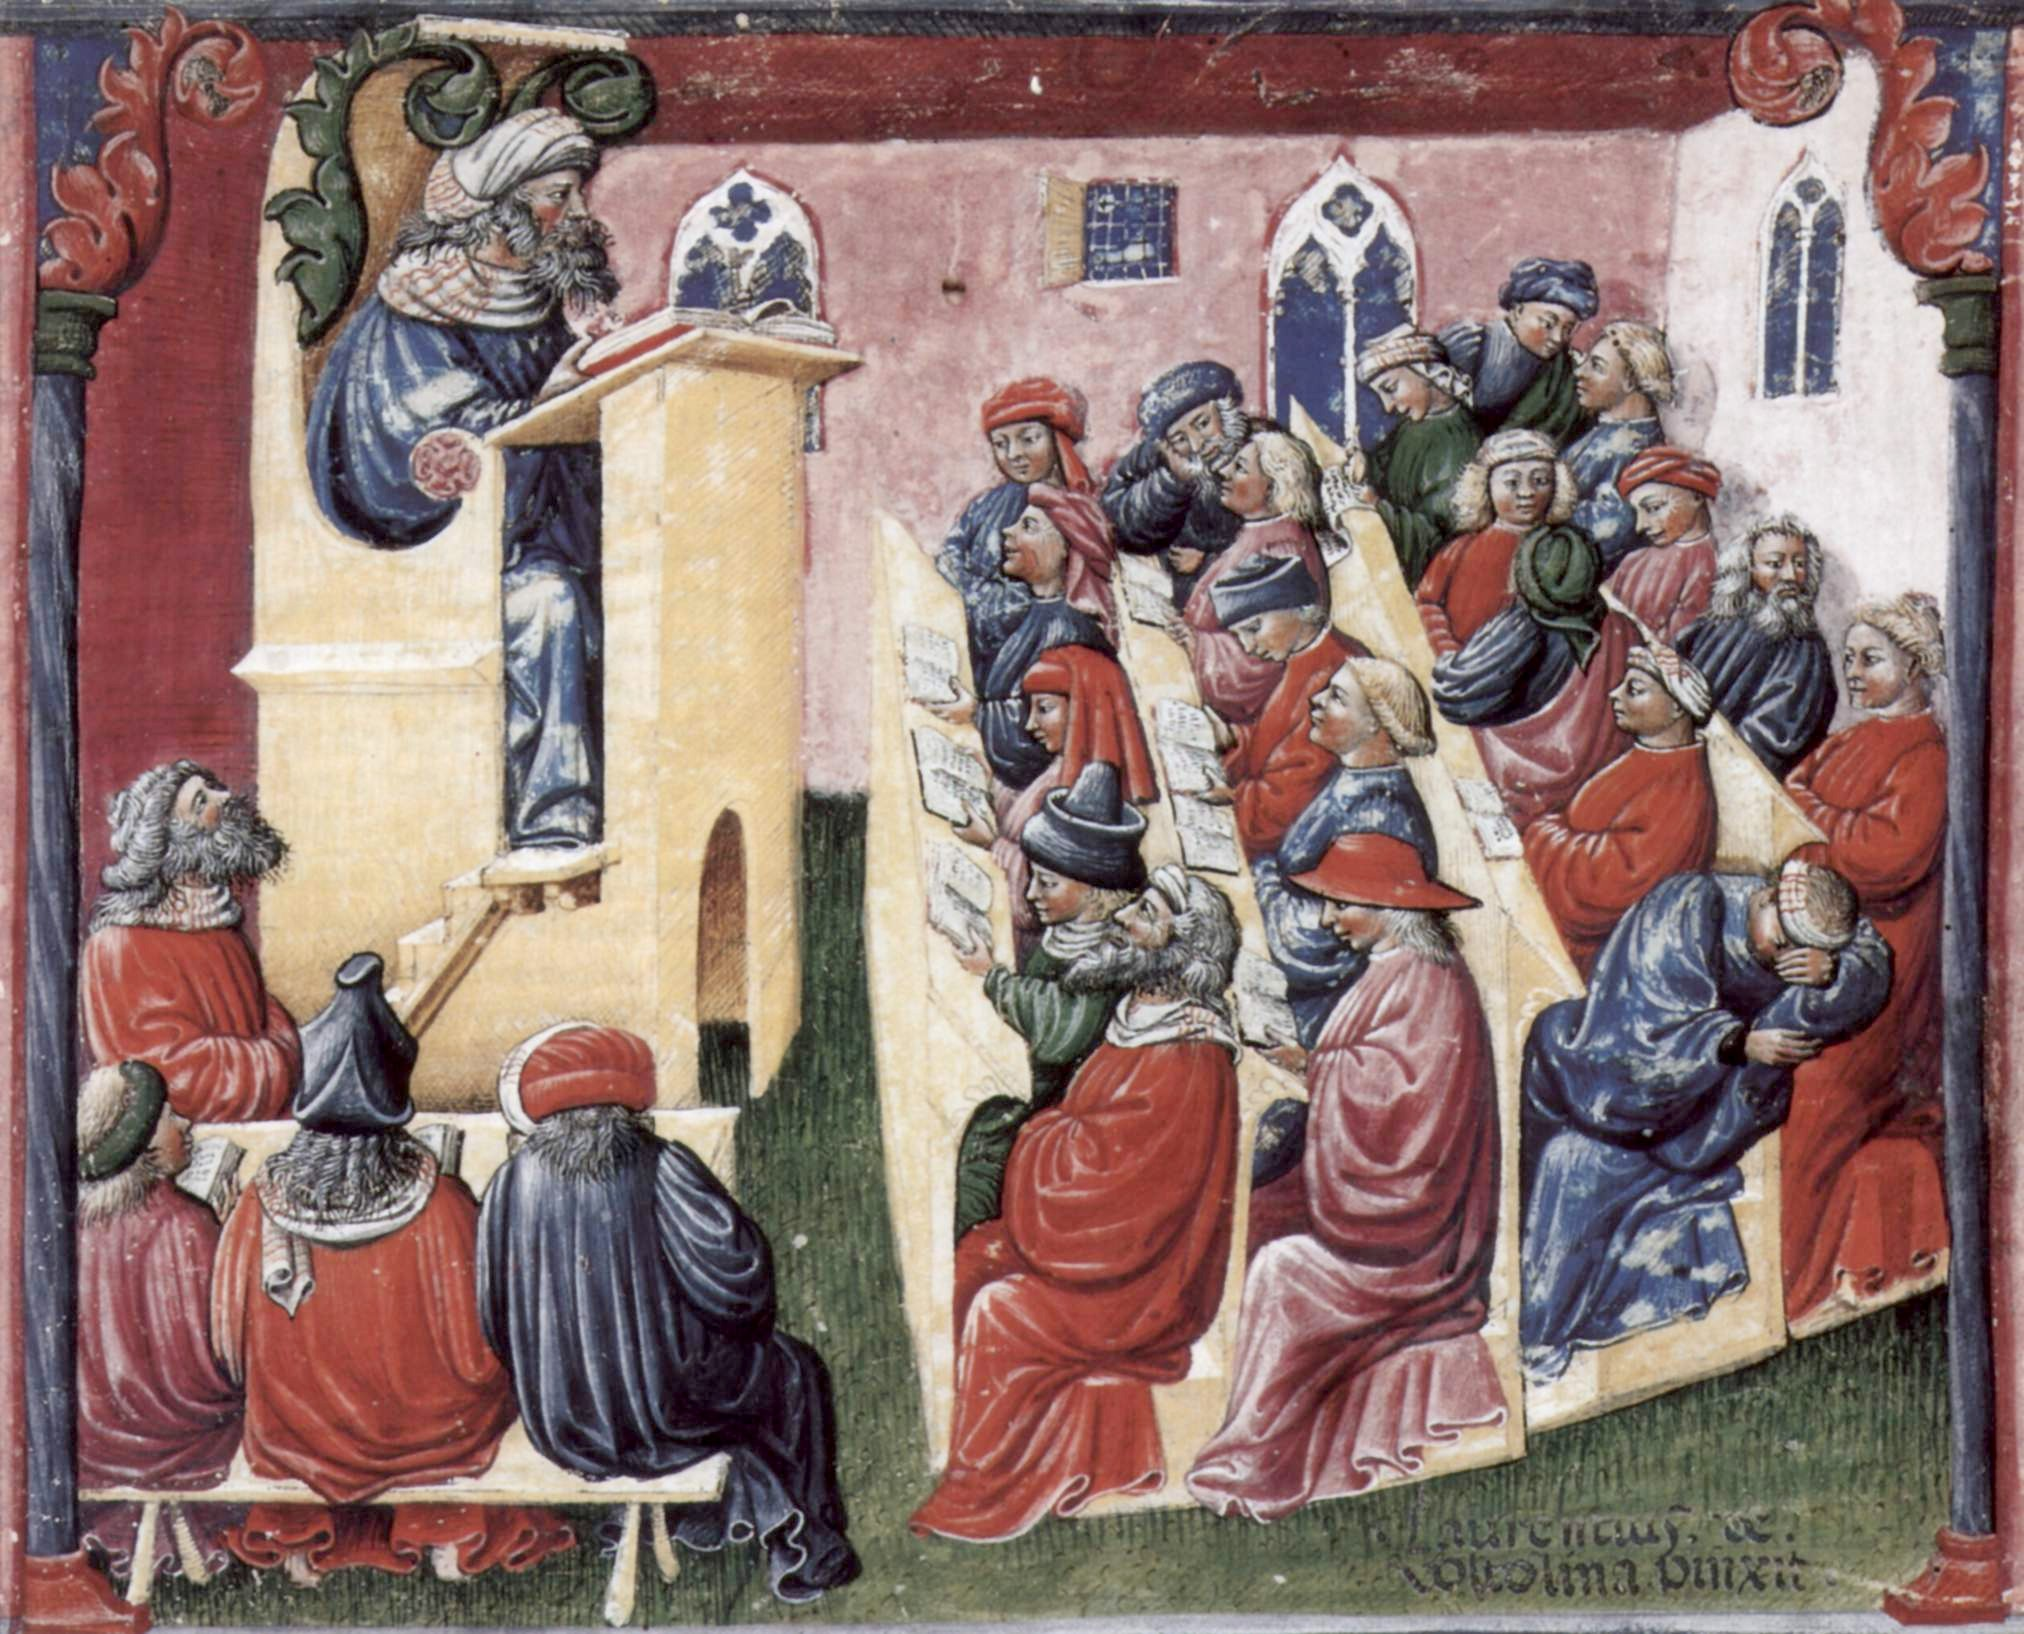
\includegraphics[width=0.65\textwidth]{laurentius.jpg}
\end{center}
{\footnotesize
Laurentius da Voltolina -- Bologna, seconda metà del XIV secolo
}
\end{frame}

%-------------------------------------------------------------------------
\begin{frame}{Riflessioni sul concetto di lezione universitaria}
	
\begin{center}
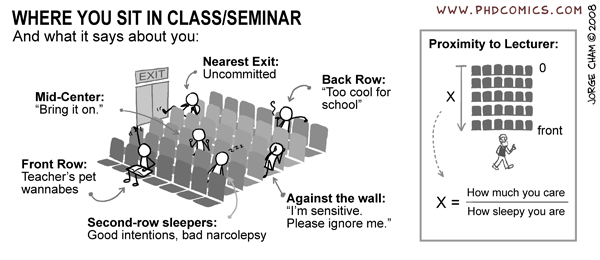
\includegraphics[width=1.0\textwidth]{wheresit.png}
\end{center}
\end{frame}

%-------------------------------------------------------------------------
\begin{frame}{Riflessioni sull'interazione a lezione}

\TwoCols{
\setlength\epigraphwidth{.90\textwidth}
\vspace{-18pt}
\epigraph{\alert{Domanda e sembrerai sciocco per un minuto, non domandare e resterai sciocco per sempre}
}{\textit{Proverbio cinese}}
}{
\setlength\epigraphwidth{.90\textwidth}
\vspace{-18pt}
\epigraph{\alert{If a listener nods his head when you're explaining your program, wake him up}
}{\textit{Alan Perlis\\Epigrams on Programming}}
}
\vspace{-12pt}
\begin{myboxtitle}[Fate domande!]
\BI
\item  Se sono poco chiaro, non esitate a chiedere ulteriori spiegazioni
\item Se volete ulteriori approfondimenti, chiedete e vi sarà dato
\item Non è detto che conosca tutte le risposte -- ma so dove cercare!
\EI
\end{myboxtitle}
\begin{myboxtitle}[Rispondete alle mie domande!]
\BI
\item Parlare in 150 è difficile, ma cercate di partecipare tutti
\EI
\end{myboxtitle}
\end{frame}


%-------------------------------------------------------------------------
\begin{frame}{Riflessioni sull'interazione a lezione}
	
\begin{center}

\includegraphics[width=\linewidth,height=\textheight,keepaspectratio]{questions.png}
\end{center}
\end{frame}


%-------------------------------------------------------------------------
\begin{frame}{Sull'uso di portatili e cellulari durante la lezione}
	
\vspace{-6pt}
\begin{center}

\includegraphics[width=1.0\textwidth]{attention.png}
\end{center}

\pause
\footnotesize
\BI
\item C. Stothart, A. Mitchum, C. Yehnert. \alert{The attentional cost of receiving a cell phone notification}. J Exp Psychol Hum Percept Perform. 41(4):893-7 (Aug. 2015).
\url{https://www.ncbi.nlm.nih.gov/pubmed/26121498}

\item A.F. Ward, K. Duke, A. Gneezy, and M.W. Bos. 
\alert{Brain Drain: The Mere Presence of One’s Own Smartphone Reduces Available Cognitive Capacity}. 
Journal of the Association for Consumer Research, 2(2):140-154 (April 2017) \\
\url{https://www.journals.uchicago.edu/doi/10.1086/691462}

\EI

\end{frame}

%-------------------------------------------------------------------------
\begin{frame}{Sull'uso di portatili e cellulari durante la lezione}

\begin{columns}[T]

\column{0.3\textwidth}
\BB{Mette il cellulare in modalità aereo}

\begin{center}
\IG{0.9}{airplane.png}
\end{center}

\column{0.3\textwidth}
\BB{Mettete il cellulare nello zaino}

\begin{center}
\IG{0.8}{backpack.jpg}
\end{center}

\column{0.3\textwidth}
\BB{Spegnete il WiFi del portatile}

\begin{center}
\IG{0.7}{wifioff.jpg}
\end{center}

\end{columns}



\end{frame}



%-------------------------------------------------------------------------
\begin{frame}{Sito web del corso}
\BB{\url{http://cricca.disi.unitn.it/montresor/asd/}}
\medskip
\TwoColsCustom{0.4}{0.58}{
\BI
\item Lucidi e appunti
\item Video lezioni
\item Software didattico
\item Esercizi e compiti passati
\item Progetti
\item Approfondimenti
\EI
}{

\includegraphics[width=1.0\textwidth]{sito-web.png}
}
\end{frame}

%-------------------------------------------------------------------------
\begin{frame}{Sito web del corso}
	
\vspace{-15pt}
\begin{center}

\includegraphics[width=1.0\textwidth]{webpage.png}


\includegraphics[width=1.0\textwidth]{style.png}
\end{center}
\end{frame}

%-------------------------------------------------------------------------
\begin{frame}{Docenti e assistenti}
	
\BIL
\item Prof. Alberto Montresor
\BI
\item Titolare: lezioni teoriche, esercitazioni
\item \underline{alberto.montresor [AT] unitn.it}
\EI
\item Dott. Cristian Consonni,  Dott. Lorenzo Ghiro
\BI
\item Esercitazioni, esercitazioni in laboratorio, correzioni progetti
\item \underline{cristian.consonni [AT] unitn.it} , \underline{lorenzo.ghiro [AT] unitn.it}
\EI
\EIL
\end{frame}

%-------------------------------------------------------------------------
\begin{frame}{Testi}


\begin{myboxtitle}[Libro adottato]
\BI
\item Bertossi, Montresor\\
\alert{\emph{Algoritmi e Strutture di Dati}}. \\
Tecniche nuove, $3^a$ ed. (2014)\\
(\euro 26.35)
\EI
\end{myboxtitle}

\begin{myboxtitle}[Approfondimenti]
\BI
\item Cormen, Leiserson, Rivest, Stein. \alert{\emph{Introduction to Algorithms}}. \\The MIT Press; $3^{\textrm{rd}}$ ed. (2009) (\euro 48.35)
\item Jon Kleinberg, Eva Tardos. \alert{\emph{Algorithm Design}}. \\Addison Wesley, $1^{\textrm{st}}$ Int. ed. (2013) (\euro 73.02)
\EI
\end{myboxtitle}

\begin{tikzpicture}[remember picture,overlay]
    \node[xshift=-1.7cm,yshift=-2.8cm] at (current page.north east){%
    \frame{
\includegraphics[width=3cm]{copertina.jpg}}};
\end{tikzpicture}

\end{frame}
%-------------------------------------------------------------------------
\begin{frame}{Lezioni e ricevimento}
	
\vspace{-9pt}
\begin{myboxtitle}[Lezioni]
\bigskip
\begin{tabular}{|l|l|l|l|}
\hline
Martedì & 15.30 -- 17.30 & Lezione/Esercitazione \textbf{or} Lab & A101 \\\hline
Giovedì & 10.30 -- 12.30 & Lezione/Esercitazione & B107 \\\hline
\end{tabular}
\end{myboxtitle}

\begin{myboxtitle}[Ricevimento]
\BI
\item Dopo ogni lezione, in aula
\item Via mail, quando volete
\item Su appuntamento	
\item Ricevimenti di gruppo, più avanti
\EI
\end{myboxtitle}
	
\end{frame}

%-------------------------------------------------------------------------
\begin{frame}{Esame}

\vspace{-9pt}
\begin{myboxtitle}[Esame diviso in due parti]
\BIL
\item \alert{50\% - Parte scritta}
\BI
\item Esame scritto (Uno per modulo/semestre) (Aula)
\item Progetti laboratorio (Uno per semestre) (Homework) 
\EI
\item \alert{50\% - Parte orale}
\EIL
\end{myboxtitle}

\begin{myboxtitle}[Calcolo voto finale x 12 crediti]
\[
\frac{\frac{\textrm{(Voto Scritto 1 + Bonus Lab1)} + \textrm{(Voto Scritto 2 + Bonus Lab2)}}{2} + \textrm{Voto Orale}}{2}
\]
\end{myboxtitle}

\begin{myboxtitle}[Calcolo voto finale x 6 crediti]
\[
\frac{\textrm{Voto Scritto + Bonus Lab + Voto Orale}}{2}
\]
\end{myboxtitle}

\end{frame}

%-------------------------------------------------------------------------
\begin{frame}{Esame scritto}

\vspace{-9pt}
\begin{myboxtitle}[Open-book]
\BI
\item \EE possibile usare libri e appunti, non strumenti elettronici
\EI
\end{myboxtitle}

\begin{myboxtitle}[Regole]
\BI
\item \alert{Salto appello}: se \underline{consegnate} lo scritto del modulo $X$, dovete saltare l'appello successivo del modulo $X$
\item \alert{Ultimo voto}: se \underline{partecipate} allo scritto del modulo $X$, l'eventuale voto già ottenuto del modulo $X$ viene perso.
\EI
\end{myboxtitle}

\begin{myboxtitle}[Compiti anni passati, con soluzioni]
\small
\url{http://cricca.disi.unitn.it/montresor/teaching/asd/materiale/esercizi/compiti/}
\end{myboxtitle}

\end{frame}
%-------------------------------------------------------------------------
\begin{frame}{Esame scritto}
\vspace{-18pt}
\IG{0.85}{grading.png}
\end{frame}
%-------------------------------------------------------------------------
\begin{frame}{Laboratorio}
	
\vspace{-9pt}
\BB{Esercitazioni di laboratorio}
\BI
\item Corrette tramite software: Contest Management System (CMS), valutate in maniera competitiva
\item Ricevete un bonus compreso fra 0 e 6 punti
\BI
\item Esercitazione 1: 13/12/2018 [0-3] punti
\item Esercitazione 2: 05/2019, [0-3] punti
\EI
\item E' obbligatorio consegnarne almeno una per poter accedere all'orale 
\EI

\end{frame}

%-------------------------------------------------------------------------
\begin{frame}{Esame orale}

Per accedere all'orale, è necessario:
\BI
\item Consegnare almeno un progetto funzionante 
\item Passare lo scritto con voto minimo 18

\begingroup
\tiny
\begin{align*}
  \mathrm{12\ crediti} & \qquad \frac{(\textrm{Voto Scritto 1 + BonusLab 1}) + (\textrm{Voto Scritto 2 + BonusLab2 })}{2} \geq 18 \\
  \mathrm{6\ crediti} & \qquad \textrm{Voto Scritto} + \textrm{Bonus Lab} \geq 18 
\end{align*}
\endgroup

\item Dopo aver passato lo scritto, potete venire all'orale quando volete
(nella stessa sessione, o in una qualunque sessione successiva)
\item Se rifiutate un voto all’orale, deve passare un mese prima di potersi ripresentare
\EI
\end{frame}

%-------------------------------------------------------------------------
\begin{frame}{Validità esami}

\vspace{-9pt}
\BB{I voti degli esami scritti non hanno  scadenza}

\medskip
\BB{I voti dei progetti non hanno scadenza}

\medskip
\BB{Caveat emptor!}
\BI
\item Se vi ripresentate fra 10 anni, non garantisco nulla....
\EI

\end{frame}

%-------------------------------------------------------------------------
\begin{frame}{Date scritti parziali}

\vspace{-9pt}
\TwoCols{
\begin{myboxtitle}[Studenti 2018/19]
\begin{tabular}{|l|l|}
\hline
Parziale 1 & Parziale 2 \\\hline
01/2019 & \\\hline
02/2019 &  \\\hline
        & {06/2019} \\\hline
06/2019 & {06/2019} \\\hline
07/2019 & {07/2019} \\\hline
09/2019 & {09/2019} \\\hline
01/2020 & {01/2020} \\\hline
02/2020 & {02/2020} \\\hline
\end{tabular}
\end{myboxtitle}
}{
\begin{myboxtitle}[Studenti precedenti]
\begin{tabular}{|l|l|}
\hline
Parziale 1 & Parziale 2 \\\hline
01/2019 & 01/2019\\\hline
02/2019 & 02/2019 \\\hline
        &    \\\hline
06/2019 & {06/2019} \\\hline
07/2019 & {07/2019} \\\hline
09/2019 & {09/2019} \\\hline
\end{tabular}
\end{myboxtitle}
}
\end{frame}

%-------------------------------------------------------------------------
\begin{frame}{Cheating policies}
	
\vspace{-9pt}
\begin{myboxtitle}[Durante gli scritti]
\BI
\item \EE vietato comunicare in qualunque modo (oralmente, in forma scritta o elettronicamente), per qualsivoglia motivo.
\item Chi viene sorpreso a parlare, viene invitato a lasciare l'aula e a ripresentarsi al prossimo appello
\item Questo vale per entrambi gli "estremi" della comunicazione: sia chi parla sia chi ascolta
\item Se avete bisogno di qualunque cosa, chiedete al docente	
\EI
\end{myboxtitle}

\begin{myboxtitle}[Dopo gli scritti]
\BI
\item Il compito potrà essere annullato anche in caso di manifesta copiatura scoperta nel corso della correzione degli scritti
\item L'annullamento riguarderà sia il “copiatore” che il “copiato”
\EI
\end{myboxtitle}

\end{frame}
%-------------------------------------------------------------------------
\begin{frame}{LEGGE 19/04/1925, n. 475 -- GU 29/04/1925 , n. 99}
	
\vspace{-9pt}
\begin{myboxtitle}[Art. 1]
“Chiunque in esami o concorsi, prescritti o richiesti da autorità o pubbliche
amministrazioni per il conferimento di lauree o di ogni altro grado o titolo
scolastico o accademico, per l'abilitazione all'insegnamento ed all'esercizio
di una professione, per il rilascio di diplomi o patenti, presenta, come
proprii, dissertazioni, studi, pubblicazioni, progetti tecnici e, in genere,
lavori che siano opera di altri, è punito con la reclusione da tre mesi ad un
anno. La pena della reclusione non può essere inferiore a sei mesi qualora
l'intento sia conseguito.”
\end{myboxtitle}
	
\end{frame}

%-------------------------------------------------------------------------
\begin{frame}{Varie ed eventuali}
    
\vspace{-9pt}
\TwoColsCustom{0.47}{0.51}{
\begin{myboxtitle}[Opportunità]
\BIL
\item ACM-ICPC
\item Google Summer of Code
\item Google HashCode
\item Hackathon(s)
\item Speck\&Tech
\item Facoltiadi
\item Coderdojo
\item Olimpiadi dell'Informatica
\EIL
\end{myboxtitle}
}{
\begin{myboxtitle}[Google Summer of Code]
\BI
\item Antonio Quartulli (2011) 
\item Federico Scrinzi (2012) 
\item Pietro Zambelli (2012)
\item Edo Monticelli (2012)
\item Savita Seetaraman (2014)
\item Emilio Dorigatti (2015)
\item Andrea Nardelli (2016)
\item Lodovico Giarretta (2016)
\item Giovanni De Toni (2017)
\item Francesco Gazzetta (2018)
\EI
\end{myboxtitle}
}

\end{frame}


%-------------------------------------------------------------------------
\begin{frame}{Contatti}

\BIL
\item Canale Telegram (annunci lezione):\\
\url{https://t.me/asd2018_19}
\item Mailing list (annunci vari, anche per ex-studenti):\\
{\small \url{https://groups.google.com/a/disi.unitn.it/forum/\#!forum/asd}}
\item Questionario valutazione didattica:\\
\url{https://goo.gl/forms/cpRZKmmJelfUomfG3}
\EIL

\end{frame}




%-------------------------------------------------------------------------
\begin{frame}{Conclusioni}
	
\IG{1.0}{lastslide.png}
\end{frame}



\end{document}